\documentclass[twocolumn,10pt]{jarticle} 
\usepackage[top=5truemm,bottom=15truemm,left=15truemm,right=15truemm]{geometry}
\usepackage[dvipdfmx]{graphicx}
\usepackage{ascmac}
%\setlength{\columnsep}{3zw}
\title{高速なログ検索エンジンHayabusaについて}
\author{あべひろし (@hirolovesbeer)}
\date{2017/12/20}
%%%%%%    TEXT START    %%%%%%

\begin{document}
\maketitle
\thispagestyle{empty}

\section{背景と目的}
ネットワークのトラブルシューティングやセキュリティインシデントに対応するため,
ネットワーク管理者はトラブルの原因を特定するためにサーバやネットワーク,セキュリティ機器から出力されるログを蓄積し,検索をすることがある.
大規模なネットワークでは,出力されるログの量も多く蓄積・検索システムの規模も巨大化する.
大量に出力される機器のログを高速に蓄積し,高速に検索するシステムとしてHayabusa\cite{hayabusa}を実装した.


\section{Hayabusaのアーキテクチャ}
%Hayabusa\cite{hayabusa}は,Interop Tokyoで収集された大量のsyslogを高速に検索するためのシステムとして設計された.
Hayabusaはオープンソースソフトウェアとして実装され,GitHub上で公開されている(https://github.com/hirolovesbeer/hayabusaa).
図 \ref{fig:hayabusa-arch} にHayabusaのアーキテクチャを示す.
\begin{figure}[h]
\centering
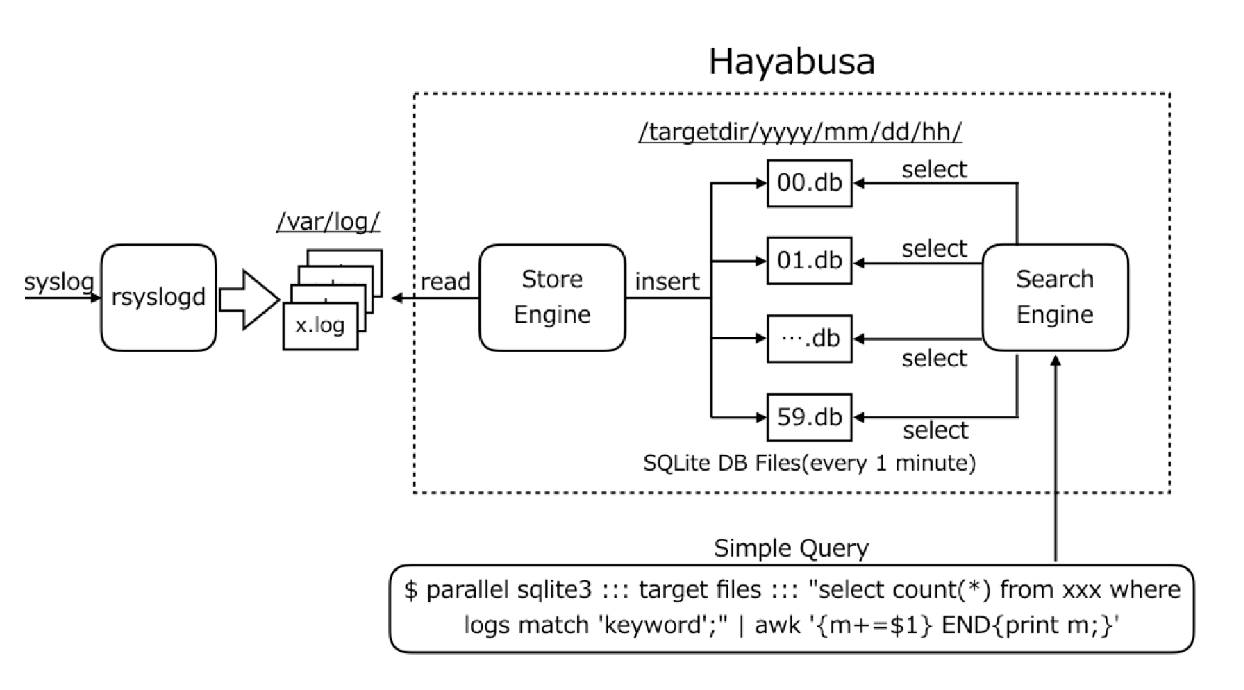
\includegraphics[width=85mm]{./pictures/hayabusa-arch.eps}
\caption{Hayabusaのアーキテクチャ}
\label{fig:hayabusa-arch}
\end{figure}

Hayabusaはスタンドアロンサーバで動作し,CPUのマルチコアを有効に使い高速な並列検索処理を実現する.
Hayabusaは大きくStoreEngineとSearchEngineの2つに分けられる.
StoreEngineはcronにより1分毎に起動され,ターゲットとなるログファイルを開きログメッセージをSQLite3ファイルへと変換する.
%ログデータは1分ごとのSQLite3ファイルへと分割され,検索時に複数プロセスにより並列処理される.
%ログが保存されるディレクトリは以下の様に時間を意味する階層として定義される.
%\begin{screen}
%\begin{verbatim}
%/targetdir/yyyy/mm/dd/hh/min.db
%\end{verbatim}
%\end{screen}
%そのためログ検索のための時間情報をデータベース内部に保持することなくディレクトリとのマッチングで行うことができ,
%時間のクエリ条件を指定することなく時間指定のログが検索可能になる.
ログが保存されるSQLite3ファイルはFTS(Full Text Search)と呼ばれる全文検索に特化したテーブルとして作成され高速なログ検索を実現する.

SearchEngineは,並列検索性能を向上させるために分単位に細分化されたFTSフォーマットで定義されたSQLite3ファイルへアクセスを行う.
各SQLite3ファイルへはGNU Parallelを用いて並列にSQL検索クエリが実行され,
結果はUNIXパイプラインを経由してawkコマンドやcountコマンドを用いて集計される.


\section{性能概要}
Hayabusaはスタンドアロン環境で動作するが,小規模なApache Sparkのクラスタよりも全文検索性能が高い.
性能評価実験では,Hayabusaは3台のApache Sparkクラスタより27倍早い検索性能を示した.
\begin{figure}[h]
\centering
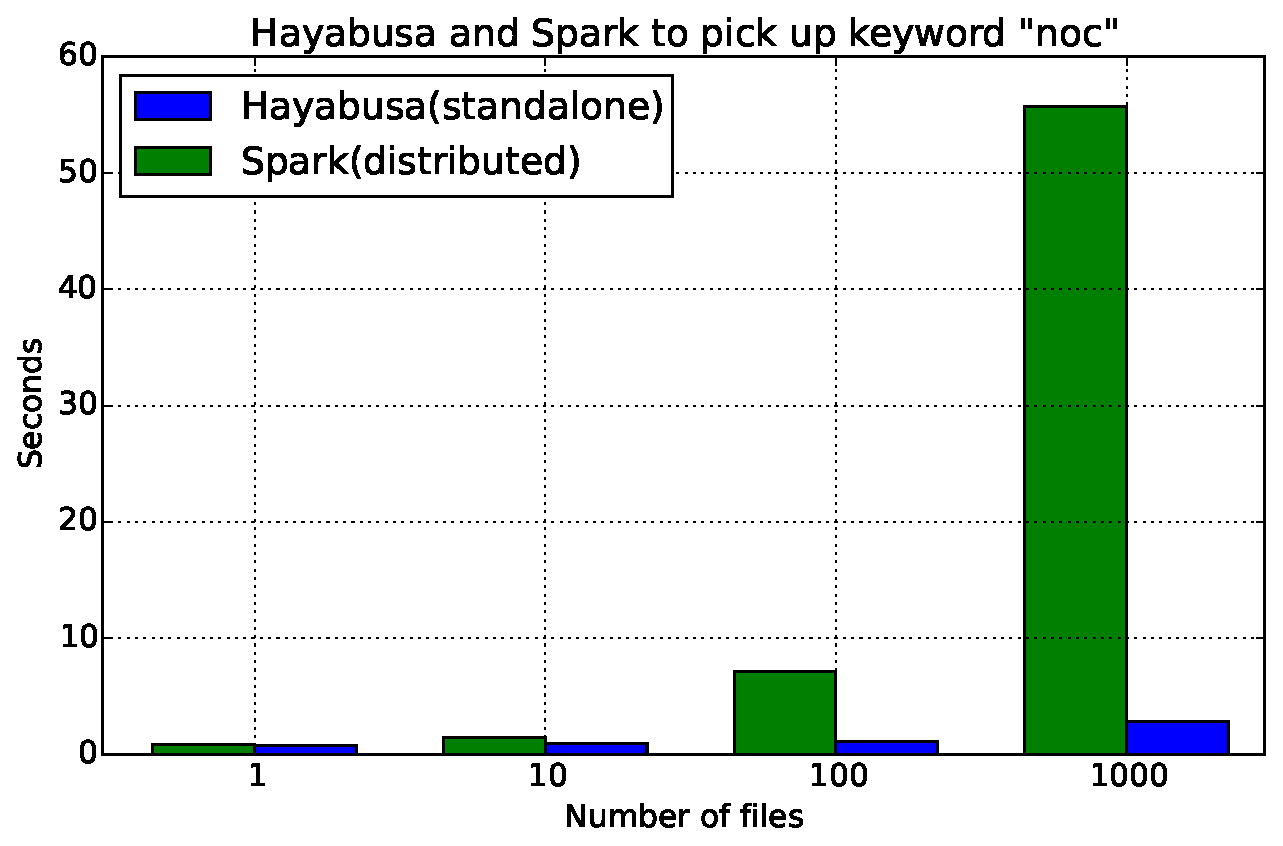
\includegraphics[width=85mm]{./pictures/spark-sqlite-dist2.eps}
\caption{HayabusaとSparkの性能比較}
\label{fig:hayabusa-spark}
\end{figure}


\section{まとめ}
スタンドアロン環境にはハードウェア限界が存在し,
規模が拡大した他の分散処理クラスタにいつかは性能が抜かれてしまう可能性が高い.
そこで,Hayabusaの限界であるスタンドアロン環境という制約を取り払い,
複数ホストでHayabusaの分散処理環境を構築し,検索性能がスケールアウトするアーキテクチャの実現をした\cite{d-hayabusa}.
計測した結果,1台の処理ホストでは約468秒かかった検索処理が最大約6秒まで短縮した.
144億レコードのsyslogデータを6秒でフルスキャンし,
全文検索可能な分散Hayabusa環境はログ検索エンジンとして高い性能を発揮する.



\begin{thebibliography}{9}
  \bibitem{hayabusa} H. Abe, K. Shima, Y. Sekiya, D. Miyamoto, T. Ishihara, and K. Okada. Hayabusa: Simple and fast full-text search engine for massive system log data., CFI’17, pages 2:1–2:7, Fukuoka, JAPAN, 2017. ACM.
  \bibitem{d-hayabusa} 阿部博 and 篠田陽一, スケールアウト可能なログ検索エンジンの実現と評価, インターネットと運用技術シンポジウム論文集 2017論文集, volume 2017, pages 73-80, nov 2017.

\end{thebibliography}


\end{document}
